
\chapter{Problemen tijdens het practicum.}


\section{Adafruit\_Microbit.h: No such file or directory.}~\\
%Adafruit_Microbit.h: No such file or directory
%Adafruit\_Microbit.h: No such file or directory.\\
Contoleer of de Adafruit microbit geïnstalleerd is.
\begin{enumerate}
	\item Ga naar de library manager zoals aangegeven in figuur \ref{fig:ardLibMan}
	\item Controleer of library geinstalleerd is, zolas aangegeven in figuur \ref{fig:ardLibCon}
\end{enumerate}

\begin{figure}[h!]
	 		\centering
	 		\begin{center} 	
		\begin{subfigure}[b]{0.45\textwidth}
     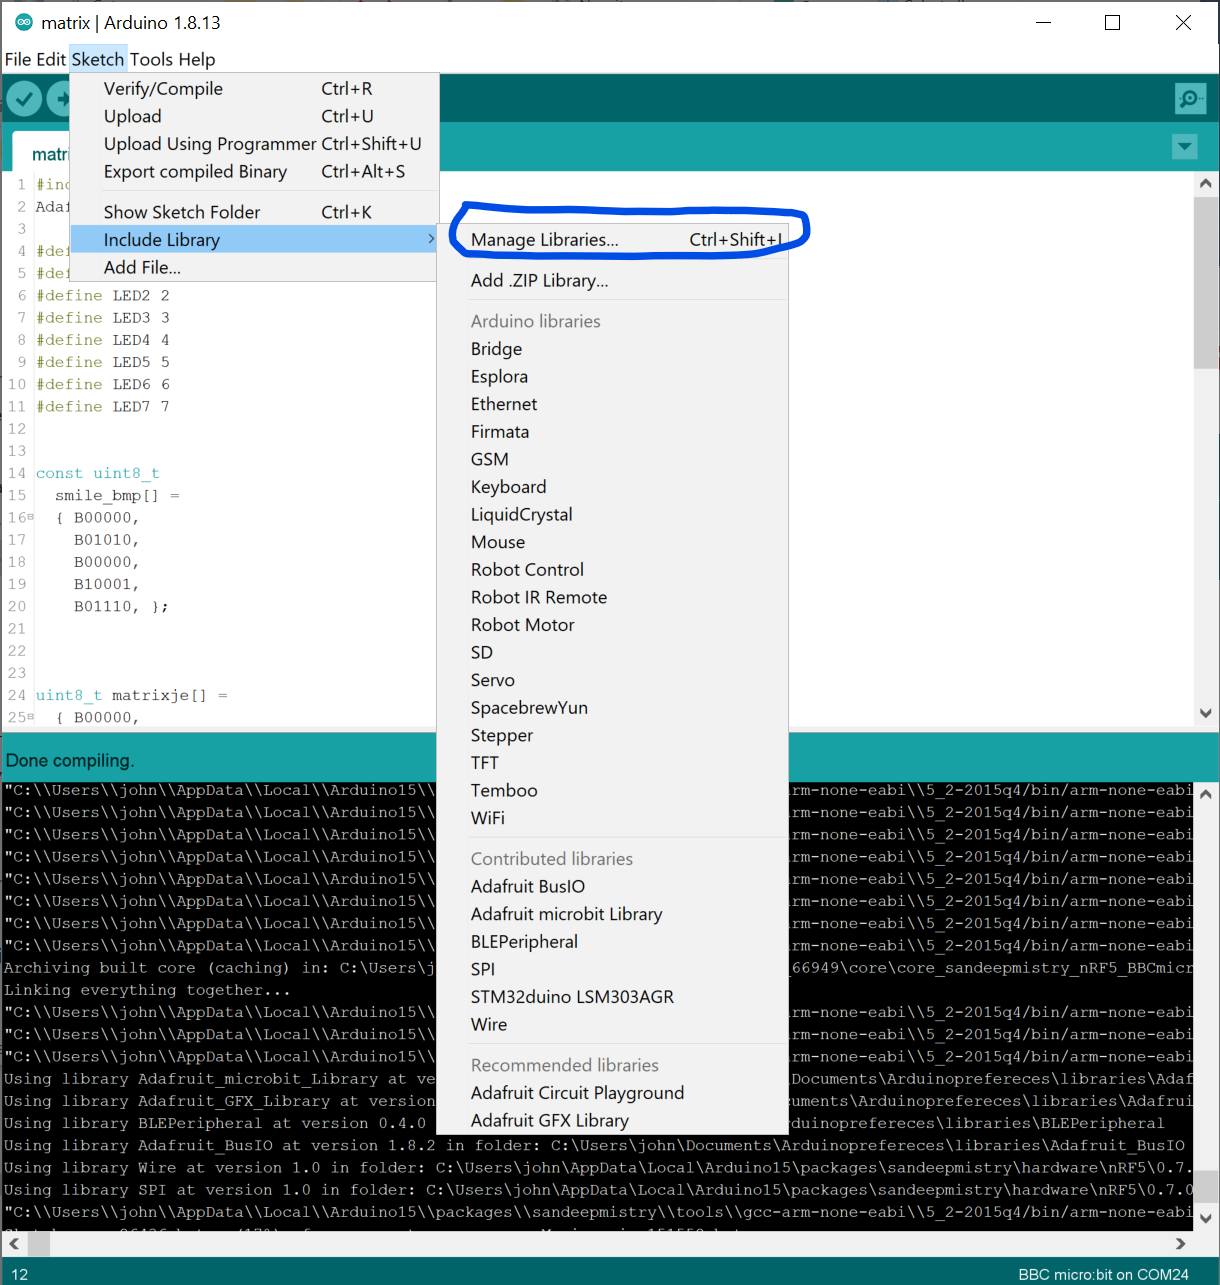
\includegraphics[width=0.7\textwidth]{figuren/arduinoManLib}
    \caption{selecteren van de library manager }
     \label{fig:ardLibMan}

\end{subfigure}
\begin{subfigure}[b]{0.54\textwidth}
	     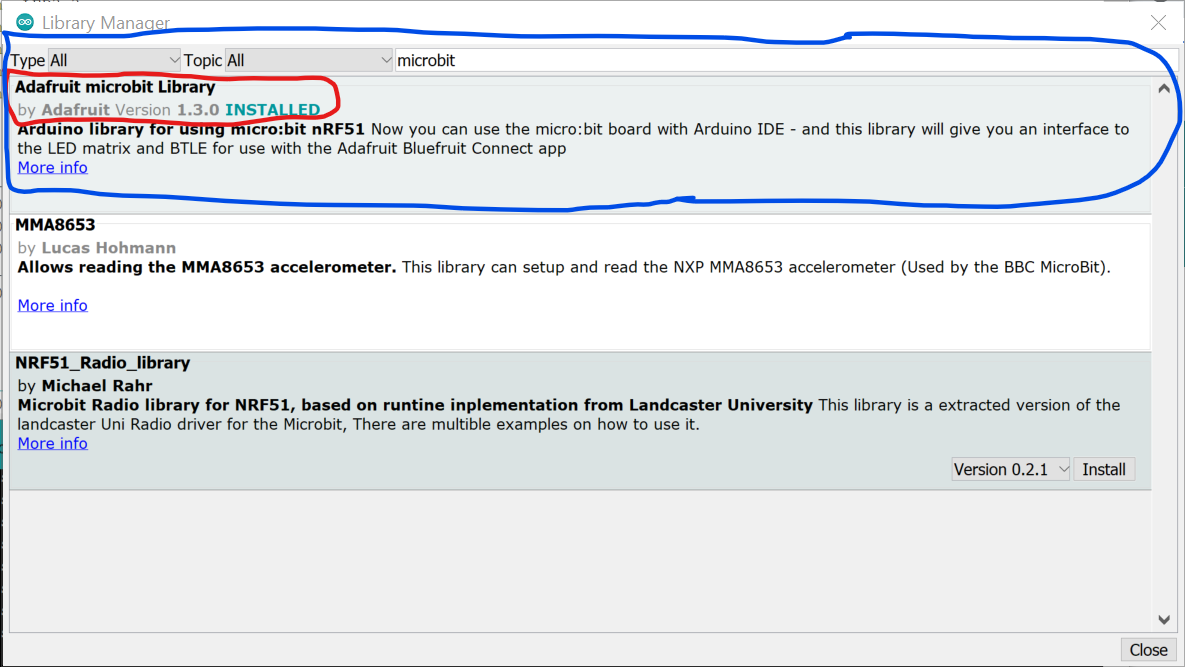
\includegraphics[width=0.98\textwidth]{figuren/arduinoManLibIns}
	\caption{Constrole Library is geïnstalleerd }
	\label{fig:ardLibCon}
\end{subfigure}
\captionsetup{justification=centering}
\caption{Controleren of library is geïnstalleerd. }
\label{fig:ardinopr1}
\end{center}

\end{figure}

\section{SerialPortException: Port name - COM..}~\\
java.io.IOException: jssc.SerialPortException: Port name - COM24; Method name - setEventsMask(); Exception type - Can't set mask.

De seriële poort is in gebruik door waarschijnlijk de monitor.

Sluit de monitor af.
 
 
\section{Tijdens het uploaden}
 Error: unable to find CMSIS-DAP device
 Error: No Valid JTAG Interface Configured.
 Error: No Valid JTAG Interface Configured.
 
 Haal de USB stekker uit de laptop en doe deze opnieuw erin.
 
 \section{Tijdens compileren  'kan stdint.h niet vinden'}
 Mogelijk is er iets fout gegaan bij het installeren van de \textbf{Add NRF5x Board Support}. Waardoor de library niet geinstalleed is.
 
 Bij het installeren van de 'Add NRF5x Board Support' moet er een lange tijd gewacht worden. Mogelijk is deze onderbroken. Bij het opnieuw installeren lijk alles goed te gaan, dit is echter niet zo.
 
 Mogelijke oplossing:\\
 remove het board en installeer deze opnieuw (wacht nu wel totdat deze geïnstalleerd is).
 
 